\documentclass[sn-apa]{sn-jnl}% APA Reference Style 
% \documentclass[sn-apa,iicol]{sn-jnl}% APA Reference Sytle with Double Column

%%%% Standard Packages
%%<additional latex packages if required can be included here>

\usepackage{graphicx}%
\usepackage{multirow}%
\usepackage{amsmath,amssymb,amsfonts}%%%
\usepackage{amsthm}%
\usepackage{mathrsfs}%
\usepackage[title]{appendix}%
\usepackage{xcolor}% shi
\usepackage{textcomp}%
\usepackage{manyfoot}%
\usepackage{booktabs}%
\usepackage{algorithm}%
\usepackage{algorithmicx}%
\usepackage{algpseudocode}%
\usepackage{listings}
\usepackage{rotating}
\usepackage{adjustbox}
\usepackage{booktabs}
\usepackage{longtable}
\usepackage{ltablex}
\usepackage{tabu}
\usepackage{verbatim}

%%%% uespackages needed for APA7 style
\usepackage[utf8]{inputenc}
\usepackage[style=apa, backend=biber]{biblatex}
\addbibresource{sn-bibliography.bib}


%% as per the requirement new theorem styles can be included as shown below
\theoremstyle{thmstyleone}%
\newtheorem{theorem}{Theorem}%  meant for continuous numbers
%%\newtheorem{theorem}{Theorem}[section]% meant for sectionwise numbers
%% optional argument [theorem] produces theorem numbering sequence instead of independent numbers for Proposition
\newtheorem{proposition}[theorem]{Proposition}% 
%%\newtheorem{proposition}{Proposition}% to get separate numbers for theorem and proposition etc.

\theoremstyle{thmstyletwo}%
\newtheorem{example}{Example}%
\newtheorem{remark}{Remark}%

\theoremstyle{thmstylethree}%
\newtheorem{definition}{Definition}%

\raggedbottom

%%\unnumbered% uncomment this for unnumbered level heads

\begin{document}

\title[Reliability of Self-Prioritization Effect as Measured by the Self-Perceptual Matching Task: Evidence from Multiple Datasets]{Reliability of Self-Prioritization Effect as Measured by the Self-Perceptual Matching Task: Evidence from Multiple Datasets}


\author[1]{\fnm{Zheng} \sur{Liu}}
\equalcont{These authors contributed equally to this work.}

\author[1]{\fnm{Mengzhen} \sur{Hu}}
\equalcont{These authors contributed equally to this work.}

\author[1]{\fnm{Yuanrui} \sur{Zheng}}

\author[2]{\fnm{Jie} \sur{Sui}}

\author*[1]{\fnm{Chuan-peng} \sur{Hu}}\email{hu.chuan-peng@nnu.edu.cn; hcp4715@hotmail.com}

\affil*[1]{\orgdiv{School of Psychology}, \orgname{Nanjing Normal University}, \orgaddress{\city{Nanjing}, \country{China}}}

\affil*[2]{\orgdiv{School of Psychology}, \orgname{University of Aberdeen}, \orgaddress{\city{Old Aberdeen}, \country{Scotland}}}


%%==================================%%
%% sample for unstructured abstract %%
%%==================================%%

\abstract{The self-prioritization effect (SPE) refers to the effect that performance on cognitive tasks is better when stimuli are related to the self than when they are not. In the last decade, the self -perceptual matching task (SPMT) has emerged as a mainstream paradigm for studying SPE due to its simplicity and elimination of familiarity effects. As a simple button-pressing task, SPMT yields two outcomes: reaction time and accuracy. Other indices can be derived from reaction times and accuracy, including sensitivity \textit{d}-prime under the signal-detection theory, the efficiency index from the direct division of RT and ACC, and drift rate (\emph{v}) and starting point (\emph{z}) estimated using the drift-diffusion models. All these indices have been used to quantify SPE in the literature. However, the reliability of these SPE indices remains unexplored. To address this research gap, we performed a pre-registered study in which we re-evaluated data from 18 datasets across 11 articles using the intraclass correlation coefficient (ICC) and split-half reliability. \textcolor{blue}{Our results reveal that response time exhibits high and consistent test-retest reliability across datasets, while accuracy-based measurements yield sub-optimal outcomes.  The ICC results suggest that all the indices related to SPE in the SPMT are more suitable for group-level analysis rather than assessing individual-level variation.} These findings establish a benchmark for future investigations utilizing the SPMT and underscore the limitations of accuracy-based measures, which should be considered when employing the SPMT as an assessment tool.}


\keywords{Self-Prioritization Effect (SPE), Self-Perceptual Matching Task (SPMT), Reliability, Multiverse}

\maketitle

\section{Introduction}\label{sec:intro}

The Self-Prioritization Effect (SPE) refers to the phenomenon whereby performance in cognitive tasks is better when stimuli are related to the self than when they are not. This effect has been widely documented and confirmed since the 1950s. In the early days of cognitive psychology, researchers found that subjects were able to recognize their own names, even when they were mixed with a noisy auditory background and not the target of the task in dichotic listening tasks \parencite{cherry1953some,moray1959attention}. SPE effect was then reported in memory research by \textcite{craik1975depth}, who found that participants were able to recall more words when they were related to the self compared to when they were processed at other levels (e.g., semantic). This SPE effect in memory was then replicated by many others \parencite{conway1995the,rogers1977self,symons1997the}. In the following decades, the SPE has also been found to occur with different stimuli, such own face \parencite{keenan2000self,kircher2000towards,turk2002mike}, own voice\parencite{hughes2013i,payne2021perceptual}, own name \parencite{constable2019it}, and newly owned object \parencite{strachan2020it}. SPE was found across a variety of cognitive tasks, such as perceptual task \parencite{cunningham2017editorial, desebrock2018self}, decision-making task \parencite{sui2013self}, attentional task \parencite{shapiro1997personal}, and ownership task \parencite{cunningham2008yours}.

Although SPE is often argued to be a self-specific effect, it can be challenging to disassociate it from the familiarity effect since most studies use stimuli owned by participants or by others. \textcite{sui2012perceptual} proposed a paradigm where participants first associate geometrical shapes (e.g., triangle, square, and circle) with labels of persons (e.g.,``You,"``friend," and``stranger") and then perform a perceptual matching task in which they decide if the shape-label pairs presented on the screen match the learned association or not \parencite{sui2012perceptual}. Because the task requires participants to learn the social meaning of different geometric shapes, it is called the Self-Perceptual Matching Task (SPMT). In this task, \textcite{sui2012perceptual} found that shapes associated with the self are performed better, with faster response times, better accuracy, and/or higher sensitivity scores, compared to shapes associated with friends and strangers. Because the self-relatedness is acquired immediately right before they start the perceptual matching task, this paradigm eliminated the effect of familiarity of the stimuli. 

Since then, the SPMT has become the mainstream method for investigating the mechanism underlying the SPE. For instance, researchers have explored the importance of personality traits in identity labels \parencite{golubickis2020parts}, the self-relevant labels that include the past, present, and future self \parencite{golubickis2017self}, as well as ``good self" and ``bad self" labels \parencite{hu2020good}, and the group advantage effect of in-group labels \parencite{constable2019relevant,constable2020sticking,enock2018self,enock2020overlap}. Moreover, the SPMT has been applied to various fields. In neuroscience and physiology, researchers investigate which brain regions are activated during self-prioritization effect \parencite{feng2018neural,humphreys2015the}, and gender differences in self-prioritization effect due to oxytocin \parencite{feng2020effect}. In clinical research, SPMT has been used to understand atypical self-processing in populations such as those with autism or depression \parencite{gillespie2018the,nijhof2019self,sui2017the}. Cross-cultural studies have shown that individuals from individualistic cultures demonstrate a stronger self-prioritization effect \parencite{jiang2019cultural}, and that the language of the experimental stimuli can affect the strength of the effect \parencite{ivaz2016the}. Finally, the SPMT has also been applied to child development, with studies examining developmental changes in self-positivity effects \parencite{maire2020a,zhou2019self}. 

While SPMT has gained widespread adoption as a prominent method for investigating the underlying mechanism of the self-prioritization effect, there has been microscopic examination and report of the psychometric properties of the outcomes, necessitating a careful evaluation \parencite{parsons2019psychological,zorowitz2023}. Given the increasing use of SPMT to assess individual differences in fields such as psychiatry \parencite{liu2022depression} and social psychology \parencite{enock2018self} it is crucial to ensure a high degree of measurement consistency to accurately assess human perceptual abilities \parencite{parsons2019psychological}. Furthermore, in tasks as simple as the SPMT, there are multiple approaches to quantify the self-prioritization effect. These include two direct measures based on SPMT, namely reaction times (RT) and accuracy (ACC), as well as derived measures such as efficiency \parencite{humphreys2015the,stoeber2008perfectionism}, \textit{d}-prime of Signal Detection Theory (SDT) \parencite{hu2020good,sui2012perceptual}, and drift rate (\textit{v}) and starting point (\textit{z}) from Drift Diffusion Model (DDM) \parencite{golubickis2017self}. Consequently, two important questions remain unanswered: (1) Do these indices reliably capture the self-prioritization effect across time points? and (2) If so, which index is most suitable for repeated measurements? Addressing these questions is crucial for establishing the reliability and validity of SPMT measurements, allowing for accurate assessment of the self-prioritization effect and its implications in various domains.

To address the existing research gap, the present study aimed to investigate the reliability of self-prioritization effect (SPE) indices in the self-perceptual matching task (SPMT). In order to comprehensively assess the SPE indices derived from SPMT, we examined six indices as mentioned earlier, that capture the disparity between self-related and other-related stimuli of the matching trials. This was achieved by reanalyzing data obtained from previous studies that employees SPMT. Given the diverse methods available for evaluating the reliability of cognitive tasks, we employed both the Split-Half Reliability and Intraclass Correlation Coefficient (ICC) to determine the reliability of each SPE index. These findings aim to provide valuable insights into the reliability and consistency of SPMT and its indices, having the potential to facilitate the future utilization of SPMT in research, clinical settings, and personal performance monitoring.


\section{Methods}\label{sec:method}

\subsection{Ethics approval}\label{subsec:ethics}

Since this research involves a secondary analysis of pre-existing data obtained from publicly available datasets or archived data from author’s group, which have used SPMT in recent years, informed consent and confidentiality are not applicable. 

\subsection{Experimental Design and Datasets}\label{subsec:experiment}
 
In order to assess the reliability of SPMT, we first provided a brief overview of its original experimental design, as described in the Experiment 1 by \textcite{sui2012perceptual}. The original SPMT used a 2 by 3 within-subject design. The first independent variable, labeled ``Matching," consisted of two levels: ``Matching" and ``Nonmatching," indicating whether the shape and label were congruent. The second independent variable, labeled "Identity," comprised three levels:``Self",``Friend", and ``Stranger", representing the corresponding identity associated with the shape.

The original SPMT consisted of two phases (see Fig. \ref{fig:SPMT_procedure}). In the first phase (learning phase), participants completed a learning task in which they associated three geometric shapes (circle, triangle and square) with three labels (self, friend, and stranger) for approximately 60 seconds. The shape-label associations were balanced across participants. In the second phase (formal experimental phase), participants completed a perceptual matching task. Each trial started with a fixation cross displayed in the center of the screen for 500 ms, followed by a shape-label pairing and fixation cross for 100 ms. the screen then went blank for 1500 ms, or until a response was made. Participants were required to judge whether the presented shape and label matched the learned associations from the learning phase and respond as quickly and accurately as possible by pressing one of two buttons within the allotted timeframe. Prior to the formal experimental phase, participants completed a training session consisting of 24 practice trials. After the training, participants completed six blocks of 60 trials in the matching task, with two matching types (matching/nonmatching) and three shape associations, for a total of 60 trials per association. Short breaks lasting up to 60 seconds were provided after each block. 

\begin{figure}[h]%
	\centering
	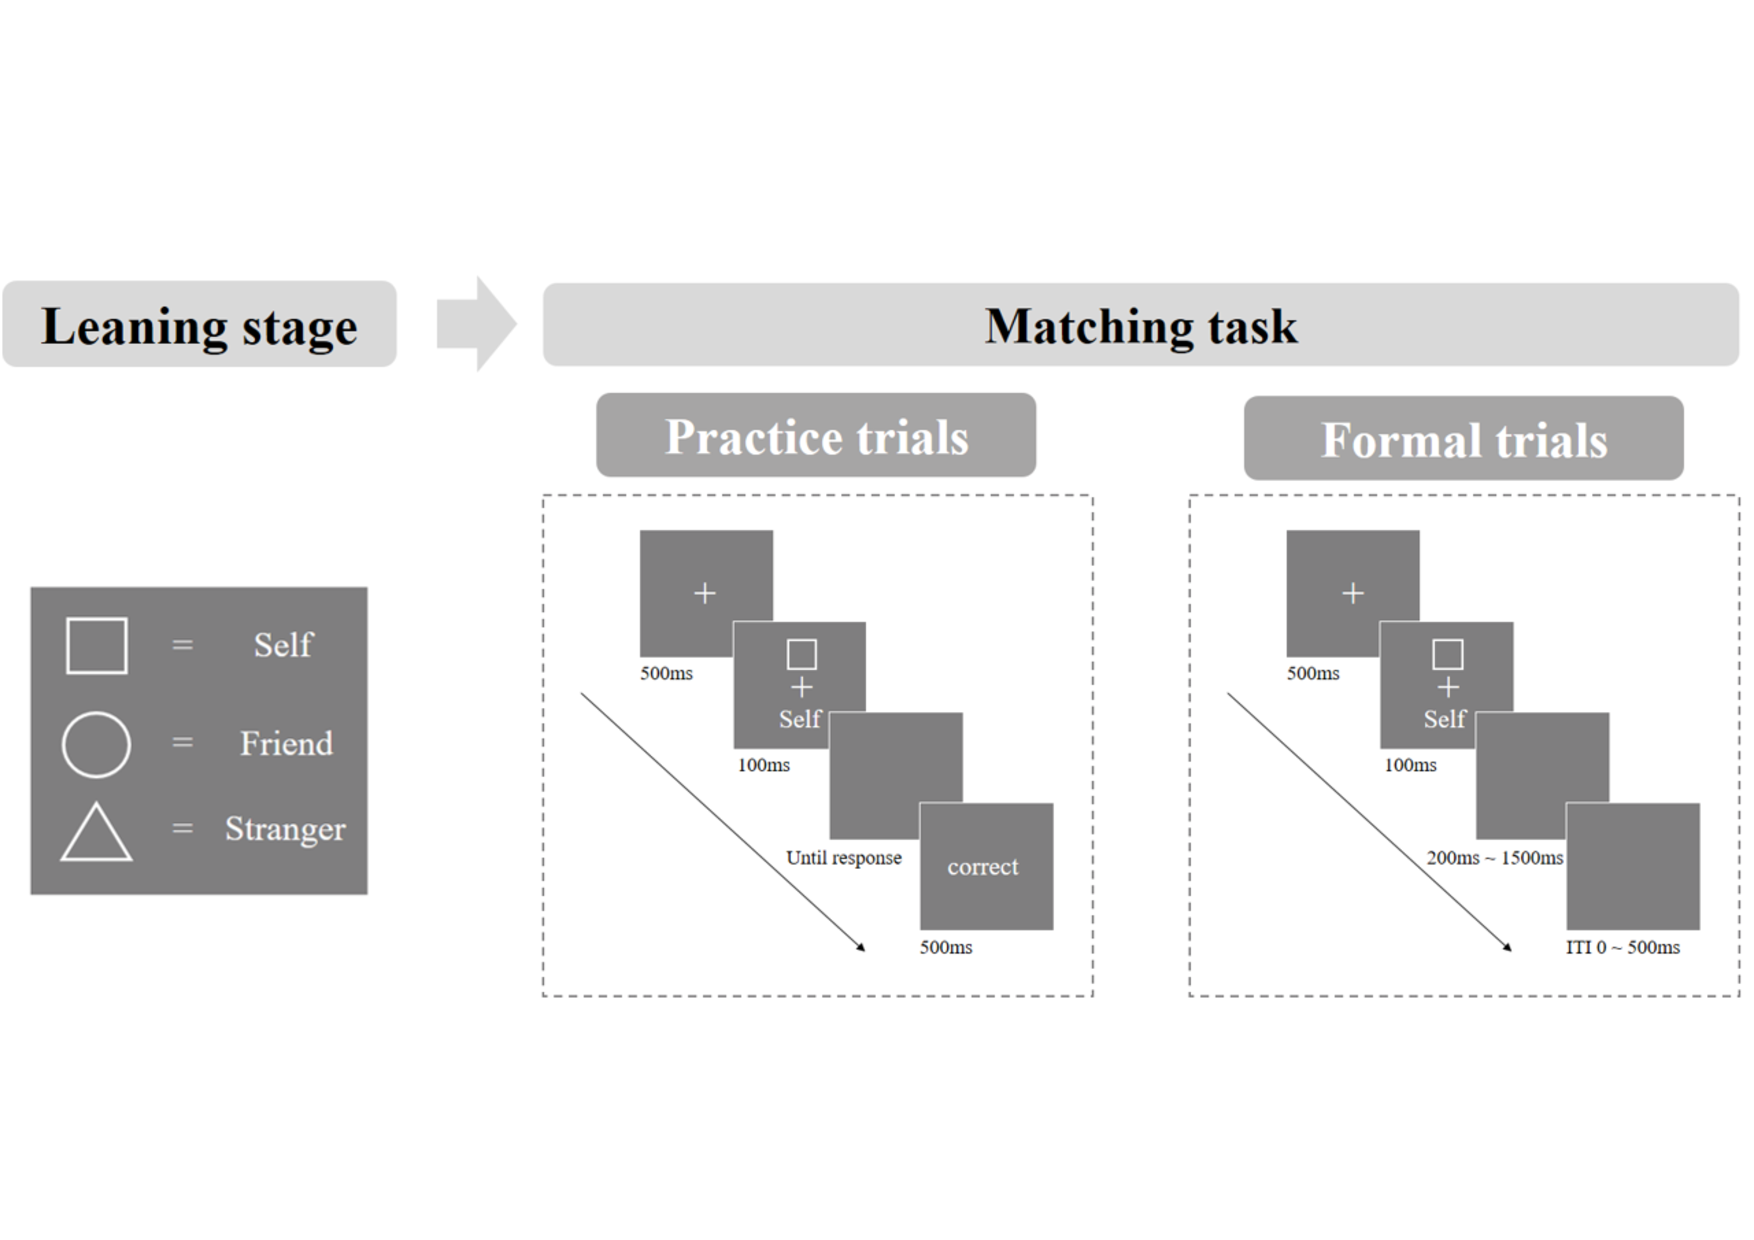
\includegraphics[width=0.9\textwidth]{./Figure/Fig_1_exp_pro.pdf}
	\caption{Procedure of the original SPMT in the Experiment 1 \textcite{sui2012perceptual}. \textit{Note}: The relation between shape-label pairs is counter-balanced between participants.
	}\label{fig:SPMT_procedure}
\end{figure}

In this study, we collected a total of 18 existing datasets derived from 11 research articles, and one from our laboratory \parencite{hu2023data} and one from our collaborators \parencite{liu2023to}, that included raw data from empirical studies utilizing the SPMT. The selection of these datasets was based on two criteria: (1) the experimental design did not deviate from the original SPMT of \textcite{sui2012perceptual}; (2) the trial-level data is available so that we can estimate at least one reliability index. All these studies shared raw data publicly \parencite{golubickis2021judging,navon2021are,qian2020prioritised,schafer2019understanding,svensson2022more} and did not deviate from the original experimental paradigm. Additionally, we identified five articles that did not have publicly available data but mentioned that data could be obtained upon request \parencite{bukowski2021socio,cheng2019saliency,kolvoort2020temporal,martinez2020examining,xu2021romantic}. One of these articles indicated that data were shared on the Open Science Framework (OSF) platform (\url{https://osf.io/pcv3u/}), but the repository was found to be empty \parencite{bukowski2021socio}. We included datasets with raw data that were accessible to us. It is worth noting that the nature of the research culture discourages direct replications \parencite{makel2012replications}; thus, all datasets included in our analysis involved some degree of modification to the original design, such as incorporating additional independent variables or using different experimental materials (see our preregistration for details). Nonetheless, not all studies incorporated repeated measures. If a publicly available datasets did not include repeated  measurements using SPMT within a specified time interval, we excluded it from calculating the Intraclass Correlation Coefficient (ICC) and only considered split-half reliability. The details of the datasets used are described in Table \ref{table:dataset}.

\begin{sidewaystable}
	\tiny
	\caption{Datasets Information}\label{table:dataset}
	\begin{tabular*}{\textwidth}{@{\extracolsep\fill}lccp{1cm}p{1cm}cccccccccccc}
		\toprule%
		&  & \multicolumn{4}{@{}c@{}}{Independent Variable} & & & \multicolumn{6}{@{}c@{}}{SPE Indices} & \multicolumn{2}{@{}c@{}}{Reliability}\\\cmidrule{3-6}\cmidrule{9-14}\cmidrule{15-16}%
		Paper & Exp. & IV 1 & IV 2\centering & IV 3\centering & IV 4 & Sample Size & \begin{tabular}[c]{@{}c@{}}
			\# of Trials\\ per Condition
		\end{tabular} & RT & ACC & d & Eff & \emph{v} & \emph{z} & ICC & SHR \\
		\midrule
		\textcite{hu2023data} & 1 & Matching & Identity\centering & 
		Emotion Control, Neutral, Happy, Sad\centering & Session & 34 & 60 & $\surd$ & $\surd$ & $\surd$ & $\surd$  & $\surd$ & $\surd$ & $\surd$ & $\surd$ \\
		\textcite{constable2020sticking} & 1 & Matching & Identity\centering & 
		Switch Identity Partner, Stranger\centering & Phase & 92 & 40 & $\surd$ & $\surd$ & $\surd$ & $\surd$  & $\surd$ & $\surd$ & & $\surd$ \\
		\textcite{constable2021affective} & 2 & Matching & Identity  Self; Stranger\centering & $--$\centering & $--$ & 51 & 24 & $\surd$ & $\surd$ & $\surd$ & $\surd$  & $\surd$ & $\surd$ & & $\surd$\\
		\textcite{qian2020prioritised} & 1 & Matching & Identity Self; Stranger; Celebrity\centering & Mood (Session)\centering & $--$ & 24 & 24 & $\surd$ & $\surd$ & $\surd$ & $\surd$  & $\surd$ & $\surd$ & & $\surd$ \\
		& 2 & Matching & Identity Self; Celebrity\centering & Cue With, Without\centering & $--$ & 25 & 50 & $\surd$ & $\surd$ & $\surd$ & $\surd$  & $\surd$ & $\surd$ & & $\surd$ \\
		\textcite{schafer2019understanding} & 1 & Matching & Identity Self, Mother, Acquaintance\centering & $--$\centering & $--$ & 103 & 24 & $\surd$ & $\surd$ & $\surd$ & $\surd$  & $\surd$ & $\surd$ & & $\surd$ \\
		\textcite{golubickis2021judging} & 1 & Matching & Identity\centering & Presentation Mixed; Blocked\centering & $--$ & 30 & 30 & $\surd$ & $\surd$ & $\surd$ & $\surd$  & $\surd$ & $\surd$ & & $\surd$ \\
		& 1 & Matching & Identity\centering & $--$\centering & $--$ & 13 & 60 & $\surd$ & $\surd$ & $\surd$ & $\surd$  & $\surd$ & $\surd$ & & $\surd$ \\
		\textcite{navon2021are} & 3 & Matching & Identity Self; Father; Stranger\centering & $--$\centering & $--$ & 27 & 60 & $\surd$ & $\surd$ & $\surd$ & $\surd$  & $\surd$ & $\surd$ & & $\surd$ \\
		& 4 & Matching & Identity\centering & $--$\centering & $--$ & 26 & 60 & $\surd$ & $\surd$ & $\surd$ & $\surd$  & $\surd$ & $\surd$ & & $\surd$ \\
		& 1 & Matching & Identity Self; Friend\centering & $--$\centering & $--$ & 20 & 50 & $\surd$ & $\surd$ & $\surd$ & $\surd$  & $\surd$ & $\surd$ & & $\surd$ \\
		\textcite{svensson2022more} & 2 & Matching & Identity Self; Friend\centering & Frequency Self $>$ Friend\centering  & $--$ & 24 & 100 & $\surd$ & $\surd$ & $\surd$ & $\surd$  & $\surd$ & $\surd$ & & $\surd$ \\
		& 3 & Matching & Identity Self; Friend\centering & Frequency Self $<$ Friend\centering & $--$ & 25 & 100 & $\surd$ & $\surd$ & $\surd$ & $\surd$  & $\surd$ & $\surd$ & & $\surd$ \\
		\textcite{cheng2019saliency} & 1 & Matching & Identity\centering & Go/No-go\centering & $--$ & 22 & 75 & $\surd$ & $\surd$ & $\surd$ & $\surd$  & $\surd$ & $\surd$ & & $\surd$ \\ 
		& 2 & Matching & Identity\centering & Go/No-go\centering & $--$ & 26 & 75 & $\surd$ & $\surd$ & $\surd$ & $\surd$  & $\surd$ & $\surd$ & & $\surd$ \\ 
		& 3 & Matching & Identity\centering & Go/No-go\centering & $--$ & 22 & 75 & $\surd$ & $\surd$ & $\surd$ & $\surd$  & $\surd$ & $\surd$ & & $\surd$ \\ 
		\textcite{bukowski2021socio} & 1 & Matching & Identity\centering & Imitation\centering & $--$ & 91 & 60 & $\surd$ & $\surd$ & $\surd$ & $\surd$  & $\surd$ & $\surd$ & & $\surd$ \\ 
		& 2 & Matching & Identity\centering & Imitation\centering & $--$ & 109 & 60 & $\surd$ & $\surd$ & $\surd$ & $\surd$  & $\surd$ & $\surd$ & & $\surd$ \\ 
		\textcite{kolvoort2020temporal} & 1 & Matching & Identity\centering & Delay, 0, 40, 120, 700\centering & $--$ & 31 & 25 & $\surd$ & $\surd$ & $\surd$ & $\surd$  & $\surd$ & $\surd$ & & $\surd$ \\ 
		\textcite{martinez2020examining} & 1 & Matching & Identity\centering & Simulation\centering & $--$ & 90 & 40 & $\surd$ & $\surd$ & $\surd$ & $\surd$  & $\surd$ & $\surd$ & & $\surd$ \\ 
		\textcite{xu2021romantic} & 1 & Matching & Identity\centering & Feedback\centering & Sex & 105 & 60 & $\surd$ & $\surd$ & $\surd$ & $\surd$  & $\surd$ & $\surd$ & & $\surd$ \\ 
		\textcite{wozniak2018prioritization} & 1 & Matching & Identity\centering & Facial Gender Male; Female\centering & $--$ & 18 & 56 & $\surd$ & $\surd$ & $\surd$ & $\surd$  & $\surd$ & $\surd$ & & $\surd$ \\
		& 2 & Matching & Identity\centering & Facial Gender Male; Female\centering & $--$ & 18 & 60 & $\surd$ & $\surd$ & $\surd$ & $\surd$  & $\surd$ & $\surd$ & & $\surd$ \\  
		\textcite{liu2023to} & 1 & Matching & Identity Self; Stranger\centering & $--$\centering & $--$ & 298 & 16 & $\surd$ & $\surd$ & $\surd$ & $\surd$  & $\surd$ & $\surd$ & & $\surd$ \\
		\botrule
	\end{tabular*}
	\footnotetext{Note: SPE: Self-Prioritization Effect, ICC: Intraclass Correlation Coefficient, SHR: Split-Half Reliability}
\end{sidewaystable}


\section{Analysis}\label{sec:analysis}

In our initial pre-registration plan, we intended to estimate the drift rate (\textit{\textit{v}}) and starting point (\textit{z}) of the drift-diffusion model (DDM) using the ``fit\_ezddm" function from the ``hausekeep" package \parencite{lin2020strong}. This function was a wrapper for the EZ-DDM function \parencite{wagenmakers2007an}. However, during parameter recovery, we discovered that the parameters provided by the``hausekeep" package differed significantly from those obtained with the original HDDM package \parencite{wiecki2013hddm} used in previous studies \parencite{golubickis2017self}. As a result, we made the decision to replace the original package with the ``RWiener" package \parencite{wabersich2014rwiener}, which we found to yield the most comparable results to the HDDM package. For detailed model comparison results, please refer to the supplementary materials. All the analyses in this paper are performed using the statistical software R \parencite{dalgaard2010r}. The research flow of the current study is visually represented in Fig. \ref{fig:roadmap}. 

\begin{figure}[h]%
	\centering
	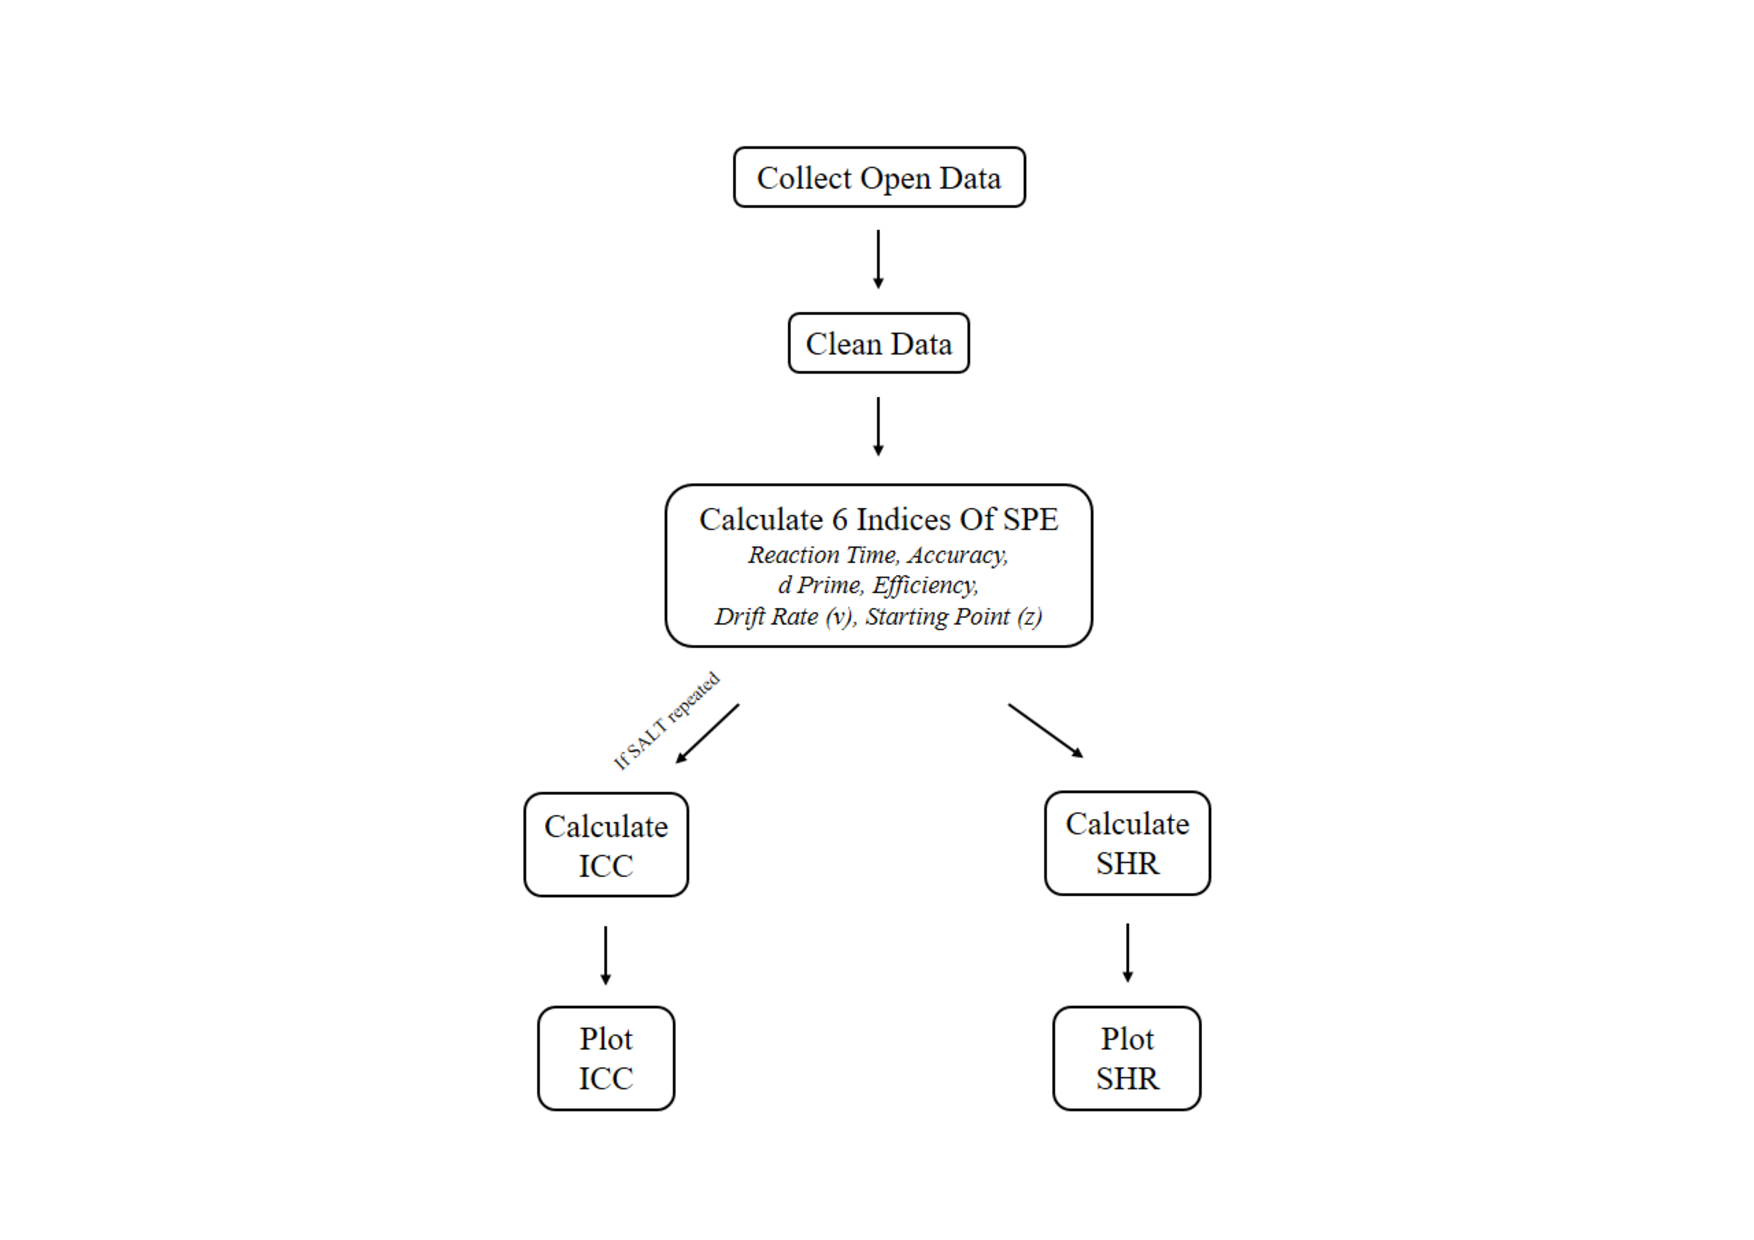
\includegraphics[width=0.9\textwidth]{./Figure/Fig_3_flow_chart.pdf}
	\caption{Roadmap of the current study. \textit{Note}: SPE: self-prioritization effect; d-prime is the sensitivity index under the Signal Detection Theory; drift rate (\emph{v}) and starting point (\emph{z}) are parameters derived from the Drift-diffusion Model; ICC: Intraclass Correlation Coefficient, SHR: Split-half Reliability.
	}
	\label{fig:roadmap}
\end{figure}

\subsection{Data Pre-processing}\label{subsec:data_preprocess}
In total, we gathered 18 publicly available datasets, as mentioned earlier and presented in Table~\ref{table:dataset}. We pre-processed the secondary data using the following criteria:
\begin{enumerate}[1.]
	\item Participant Exclusion Criteria
	
	 (\romannumeral1)~Participants who had wrong trial numbers because of procedure errors is excluded from the analysis, 
	 
	 (\romannumeral2)~Participants with an overall accuracy $< 0.5$ is excluded from the analysis, 
	 
	 (\romannumeral3)~Participants with any of the conditions with zero accuracy is excluded from the analysis.
	 
	\item Behavioural Data Exclusion Criteria
	
	(\romannumeral1)~Trials with no response or wrong key press is excluded from the analysis,
	
	(\romannumeral2)~The practice trials is excluded from the formal analysis,  
	
	(\romannumeral3)~Participants with any of the conditions with zero accuracy is excluded from the analysis,
	
	(\romannumeral4)~The data under conditions other than the ``control condition'' would not be used in the current study. 
\end{enumerate}

\subsubsection{Calculation of SPE}\label{subsubsec:SPE_Calcu}
For each dataset, we calculated six indices for each experimental condition: Mean RT (MRT), accuracy (ACC), \textit{d}-prime ($d'$), efficiency ($\eta$), drift rate (\textit{v}), and starting point (\textit{z}). Mean RT and ACC are obtained directly from the datasets, while $d'$ and $\eta$ are calculated based on Mean RT and ACC using a simple formula (see Table \ref{table:SPEcal}). 

\begin{sidewaystable}
	\caption{Indices in SPMT and corresponding SPE calculation}
	\label{table:SPEcal}%
	\begin{tabular}{@{}lccp{4cm}@{}}
		\toprule
		Indices & Indices Calculation & SPE Calculation Based on Indices & Source \\
		\midrule
		Mean RT (MRT)    & Total RT/Total Responses   & $\text{RT}_{\text{other-matching}}-\text{RT}_{\text{self-matching}}$  & \textcite{sui2012perceptual}  \\
		Accuracy (ACC)    & \# of Correct Responses/Total Responses  & $\text{ACC}_{\text{self-matching}}-\text{ACC}_{\text{other-matching}}$  & \textcite{sui2012perceptual}  \\
		\textit{d}-prime ($d'$)    & $\mathcal{Z}\left(\text{Hits}\right)-\mathcal{Z}\left(\text{False Alarms}\right)$   & $\text{$d'$}_{\text{self-matching}}-\text{$d'$}_{\text{other-matching}}$  & \textcite{sui2012perceptual} \\
		Efficiency ($\eta$)& MRT/ACC   & $\text{$\eta$}_{\text{self-matching}}-\text{$\eta$}_{\text{other-matching}}$  & \textcite{humphreys2015the,stoeber2008perfectionism}  \\
		Drift Rate (\textit{v})  & \multirow{2}{*}{Parameters decomposed from RT based on DDM}   & $\text{$v$}_{\text{self-matching}}-\text{$v$}_{\text{other-matching}}$  & \textcite{golubickis2017self}  \\
		Starting Point (\textit{z})  &  & $\text{$z$}_{\text{self-matching}}-\text{$z$}_{\text{other-matching}}$   & \textcite{golubickis2017self}  \\
		\botrule
	\end{tabular}
	\footnotetext{Note:  $\mathcal{Z}(\cdot)$ denotes the calculation of Z-score. In this context, "hit" refers to the ACC in matching trials, while "false alarm" refers to the error rate (1- ACC) in mismatch trials.}
\end{sidewaystable}



\subsubsection{Estimating the Reliability}\label{subsubsec:reliability}
\textbf{Split-half reliability.} We calculated the split-half reliability of the six indices using four types of split-half reliability measures: odd-even, front-back, permutation, and Monte Carlo \parencite{kahveci2022reliability,pronk2022methods}. The odd-even split divides trials into odd and even numbered sequences, while the front-back split divides the first and second halves of trials. The permutation split shuffles the trial order and randomly assigns each half to a group. The Monte Carlo split-half is similar to the permutation split-half, but it repeats the process thousands of times to calculate the average and 95\% confidence interval of the split-half reliability. This study will primarily use Monte Carlo split-half to determine the split-half reliability of SPMT for its robustness \parencite{pronk2022methods}. The results of the other three split-half methods is presented in the supplementary materials.

First, the data is stratified according to Session (if applicable), Matching, and Identity. If the data is not stratified, directly splitting it in half will result in an uneven distribution of trials for each experimental condition in the two halves, which can lead to an overestimation or underestimation of split-half reliability. Therefore, once the data is stratified, we split it into two halves. For example, when using Monte Carlo Split-Half, we randomly split the data into two halves. Then we repeat this process 1000 times. This will result in 1000 pairs of two halves of the data. Next, we use these 1000 pairs of data to calculate 1000 Pearson correlation coefficients, and then obtain the average and 95\% confidence interval of the Monte Carlo split reliability. First-second split, odd-even split, and permutated split are similar to Monte Carlo method, but they only perform one split, so only one split-half reliability is obtained without an interval estimate of the split-half reliability.

\textbf{Test-Retest Reliability (ICC).} We assessed the test-retest reliability of the six indices in our dataset that involved multiple experiment sessions by calculating the Intraclass Correlation Coefficient (ICC). To perform this analysis, we utilized the ``psych" package as described by \parencite{revelle2017psych}. ICC is a well-established measure used in test-retest, intra-rater, and inter-rater studies to assess reliability \parencite{fisher1992statistical}. Unlike the Pearson correlation coefficient, ICC takes into account both the correlation and agreement between multiple measurements, making it a more comprehensive measure of test-retest reliability. Within the ICC family, we specifically employed ICC2 and ICC2k. ICC2 focuses on the individual-level reliability of the indices, while ICC2k evaluates the reliability of mean ratings furnished by a group of judges \parencite{koo2016a,liljequist2019intraclass}. For the calculation of ICC2 estimates, the formula is: 
\begin{equation}
	\text{ICC2}=\frac{M S B S-M S E}{M S B S+(k-1) M S E+\left(\frac{k}{n}\right)(M S B M-M S E)},
\end{equation}
where \textit{MSBS} is the mean square between subjects, \textit{MSE} is the mean square error, \textit{MSBM} is the mean square between measurements, \textit{k} is the number of measurements, \textit{n} is number of participants. For the calculation of ICC2k estimates, the formula is: 
\begin{equation}
	\text{ICC2k}=\frac{M S B S-M S E}{M S B S+\left(\frac{M S B M-M S E}{n}\right)}.
\end{equation}

Although there is no strict criterion for defining the level of reliability, a widely accepted guideline for Cronbach's alpha is that a value of 0.60 is``acceptable", and a value greater than 0.8 means excellent reliability \parencite{cicchetti1981developing,kupper2020on}. 

\section{Results}\label{sec4}
\section{Discussion}\label{sec5}

Evaluating the reliability of a behavioral paradigm is essential for researchers planning to use the paradigm to investigate different research questions, such as individual differences and underlying mechanisms. However, despite its importance, this practice is not yet widely adopted \parencite{hedge2018reliability, parsons2019psychological,green2016use}. In this pre-registered study, our objective is to investigate the reliability of the indices related to the self-prioritization effect (SPE) in the self-perceptual matching task (SPMT). We  re-analyzed data from 18 datasets across 11 articles by employing the intraclass correlation coefficient (ICC2,ICC2k) and split-half reliability for this purpose. Our analysis of these datasets collectively demonstrate that RT yield better results compared with other indices, and the result varies between different associations. The test-retest reliability results suggest that Response time (RT) and efficiency score consistently exhibits high ICC2k and low ICC2 across datasets (xxx). However, measurements based on accuracy and DDM yield varying outcomes. Overall, the indices related to the SPE in the SPMT are more suitable for group-level analysis rather than assessing individual-level variation.

In terms of split-half reliability, the results indicate variations between the target and indices. Specifically, RT yields superior results compared to other indices, suggesting it is the most reliable indicator for accurately assessing and distinguishing between the self and other targets in the SPMT. Furthermore, when examining the split-half reliability for the self-other difference, self-stranger is the highest among other comparisons. Such finding suggests that the measurement of this particular difference remains consistent across participants and studies, indicating the systematic processing difference. The self-friend differences demonstrate the lowest reliability, indicating that the measurements obtained from the indices are not stable or consistent when split into two halves. This finding suggests that distinguishing between the self and friend in the paradigm is challenging. The aforementioned result aligns with previous studies conducted using SPMT, consistently demonstrating the establishment of a reliable self-advantage. This advantage is observed when the shapes are associated with the self, in comparison to when they are linked to an unfamiliar person or a neutral label\parencite{sui2012perceptual,feng2020effect}. 

Although RT yield the highest split-half reliability among other indices, the result is still below a commonly considered excellent reliability (). The low test-retest reliability may suggest that the indices in SPMT is subject to random error and inconsistent performance. Several plausible reasons can be identified. Firstly, a potential contributor to low split-half reliability could be the insufficient number of trials per condition. A recent study by \textcite{kucina2023calibration} has highlighted the significance of the number of trials in cognitive tasks for determining reliability. The findings of the study revealed that increasing the number of trials resulted in greater magnitudes of conflict effects and individual differences. Consequently, this led to improved reliability when compared to previous archival data. Specifically, in the case of gamified Flanker task, the study identified that achieving satisfactory reliability required 48 or fewer trials, while achieving a higher level of reliability necessitated 72 trials. Therefore, incorporating a higher number of trials in future employment of the SPMT paradigm may enhance the split-half reliability by enhancing the consistency of measurement. Second, it is worth mentioning the influence of serial dependence effects on task reliability. A recent set of studies has examined serial dependence effects in a variety of cognitive tasks \parencite{zhang2020individual, braun2018adaptive}. SeriAal dependence refers to the phenomenon in which the outcome of one trial is influenced by preceding trials, resulting in a systematic relationship between consecutive trials \parencite{pascucci2023serial}.  Notably, studies in the field of perceptual decision making have demonstrated strong serial dependence effects in perception, even when the visual stimuli were reliable and varied randomly over time \parencite{fischer2014serial,john2016serial}. In particular, if the split-half design unintentionally separates temporally adjacent trials in the SPMT, the presence of serial dependence may introduce performance differences between the halves, leading to a reduction in the reliability estimate. Thus, to accurately control for the impact of serial dependence in experiments, further research should employ appropriate statistical methods that account for the temporal dependencies between trials. Time series analysis techniques \parencite{huitema1986autocorrelation} or modeling approaches that capture the serial correlation \parencite{mei2023using} can be utilized to obtain more accurate results. 


%%We observed that certain indices we tested demonstrated good to excellent group-level test-retest reliability (ICC2k). Specifically, the RT index exhibited an ICC of 0.77, while the Efficiency measures of the SPMT task showed an ICC of 0.74. However, individual-level test-retest reliability results indicated poor performance across all indices, with ICC2 values ranging from 0.2 to 0.4. 
The discrepancy between the high ICC2k and low ICC2 suggests that thew SPMT is more influenced by between-participant variability than within-participant variability \parencite{hedge2018reliability,liljequist2019intraclass}. It is common for behavioral paradigm to have such result pattern, as demonstrated in previous research testing other cognitive paradigms such as Flanker, Simon, or Stroop \parencite{clark2022test,mollon2017individual}. There are various reasons for this pattern. First, one significant factor could be the prevalence of practice effect, particularly if the practice effect is large enough to cause a substantial change in participants' performance between measurement occasions, it can introduce additional variability in the measurements. This increased variability may lower the ICC2 \parencite{oswald2015development,siegelman2017measuring}. The presence of a practice effect underscores the need for alternative measures that can consistently capture performance nuances and reveal individual differences more sensitively \parencite{hedge2018reliability}. To address this limitation, researchers can consider incorporating additional performance metrics, such as composite RT-accuracy scores. By including RT alongside accuracy, a more stable  assessment of participants' abilities can be achieved, allowing for greater ICC2. Second, behavioral paradigms are susceptible to factors such as external conditions, contextual differences etc.., which contribute to greater within-participant variability and lower ICC2 values. However, when averaging performance between different individuals, the task could still exhibit good consistency, resulting in higher ICC2k values. It's important to note that low ICC values should not be solely interpreted as a measure of a test's overall quality but rather as an indication of the types of questions it can effectively address. In practical terms, the results suggest that the SPMT is better suited for distinguishing performance differences between individuals or groups, rather than capturing consistent performance within the same individuals over time. Thus, the SPMT may be particularly useful for studying inter-individual variability or conducting group-level comparisons, rather than tracking individual-level changes or stability. Therefore, we recommend that researchers take these factors into consideration when investigating individual differences in performance using the SPMT.

Our study has a few limitations that should be acknowledged. Firstly, although we made efforts to enhance sample diversity by including open data as much as possible, it is important to note that a majority of our samples still consisted of individuals from what is commonly referred to as``wired" populations \parencite{rad2018toward}. Therefore, our findings may not be fully representative of the broader population, and a more diverse sample is needed to ensure greater generalizability. Additionally, it is important to highlight that the majority of the studies included in our analysis focused on adults from healthy populations. Hence, further investigation is needed to determine the reliability of the SPMT across different age groups and clinical populations.Secondly, it is important to clarify the aim of our study, which primarily focused on exploratory purposes and providing information regarding the current state of reliability for the assessed indices. Consequently, it is recommended that future research focuses on modifying the paradigm and conducting tests to assess potential improvements. We propose several approaches that could be considered, such as introducing more challenging task variations, which have the potential to increase the reliability of accuracy measurements. Another suggestion is to include a greater number of trials for each condition, as this may contribute to improved reliability. It is strongly encouraged to undertake further investigation and experimentation in order to refine the paradigm and enhance the reliability of the indices, rather than dismissing the paradigm under certain circumstances.

In conclusion, the current study find that RT-base measurements proved more robust than accuracy ones. Moreover, SPMT is more suitable for group-level analysis rather than assessing individual-level variation. The findings of our study offer significant insights into the reliability of SPMT, shedding light on important factors that require careful consideration when interpreting the reliabilities. These findings also have implications for future task design and data collection protocols aimed at improving reliability. Ultimately, our study paves the way for the prospective utilization of these tasks, in various domains including research, clinical applications, and personal performance monitoring. The information obtained from our study contributes valuable knowledge to the field and sets the stage for further investigations and advancements in utilizing SPMT effectively.




%%\section{Conclusion}\label{sec13}

%%Conclusions may be used to restate your hypothesis or research question, restate your major findings, explain the relevance and the added value of your work, highlight any limitations of your study, describe future directions for research and recommendations. 

%%In some disciplines use of Discussion or 'Conclusion' is interchangeable. It is not mandatory to use both. Please refer to Journal-level guidance for any specific requirements. 

%%\backmatter

\section*{Acknowledgments}

The present research is support by xxx. 

\section*{Author Contributions}

HCP contributed to the conception and supervision of the study. JS contributed to fund raising, HCP contributed to data collection. ZL, ZYR and HMZ performed the data pre-processing, analysis and visualize the results. In addition, ZL, JS, HMZ and HCP contributed to the discussion of the results and the drafting of the final manuscript. All authors critically revised the manuscript.

\section*{Data and Material Availability}

The pre-registration plan is available at \url{https://osf.io/zv628}. The de-identified raw data from our lab (Dataset 0) is available at \url{https://doi.org/10.57760/sciencedb.08117}. The simulated data is accessible on GitHub (\url{https://github.com/Chuan-Peng-Lab/ReliabilitySPE}). 

\section*{Code Availability}

Code used to simulate and analyze the data is made accessible at \url{https://github.com/Chuan-Peng-Lab/ReliabilitySPE}. 

\section*{Competing Interests}

The authors declare no competing interests.

\section*{Supplementary information}




%%===========================================================================================%%
%% If you are submitting to one of the Nature Portfolio journals, using the eJP submission   %%
%% system, please include the references within the manuscript file itself. You may do this  %%
%% by copying the reference list from your .bbl file, paste it into the main manuscript .tex %%
%% file, and delete the associated \verb+\bibliography+ commands.                            %%
%%===========================================================================================%%


\printbibliography
%\bibliography{sn-bibliography}% common bib file
%% if required, the content of .bbl file can be included here once bbl is generated
%%\input sn-article.bbl
\end{document}
